\chapter{Results and Discussion}
\label{ch:results}

In this chapter, I present the results of the trend detection experiment
described in chapter \ref{ch:data}. I show the quality of the trend detection
algorithm using ROC curves and distributions of detection time relative to the
true trend onset. I analyze the effect of the algorithm parameters on the
tradeoff between false positive rate, true positive rate, and relative detection
time. Finally, I propose parameter regimes appropriate for three situations: 1)
the cost of a false positive outweighs the cost of a false negative, 2) the cost
of a false negative outweighs the cost of a false positive, and 3) the costs of
a false positive and a false negative are comparable.

\section{ROC Curve Envelopes}

Figures \ref{fig:roc_env1} and \ref{fig:roc_env2} shows the false positive
rates ($FPR$) and true positive rates ($TPR$) that result from varying each
detection parameter, aggregated over all combinations of the remaining
parameters. The left side of each plot shows a scatter plot of false positive
and true positive rates, while the right side shows the upper-left-most envelope
of the set of all ROC curves.

%TODO: Uncomment
\begin{comment}
\begin{figure}[!h]
\begin{center}
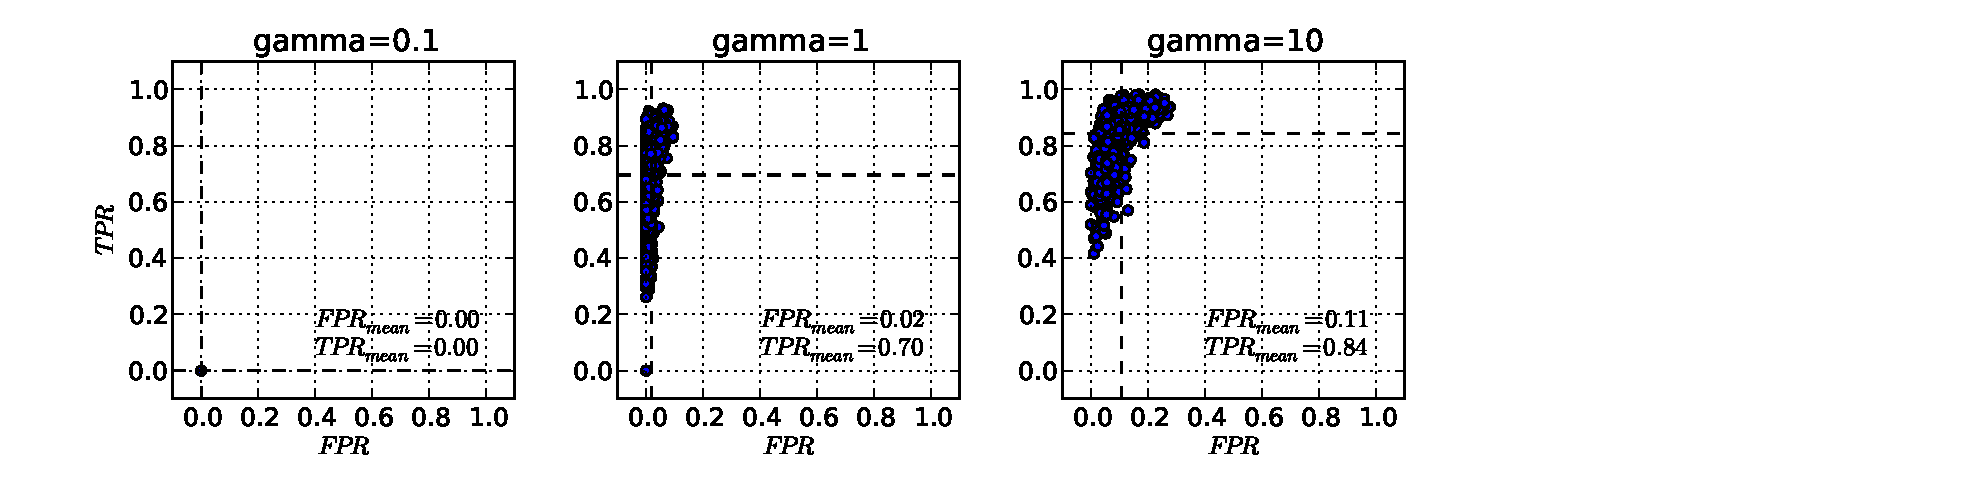
\includegraphics[height=2.5in]{../fig/final/scatter_env/gamma}
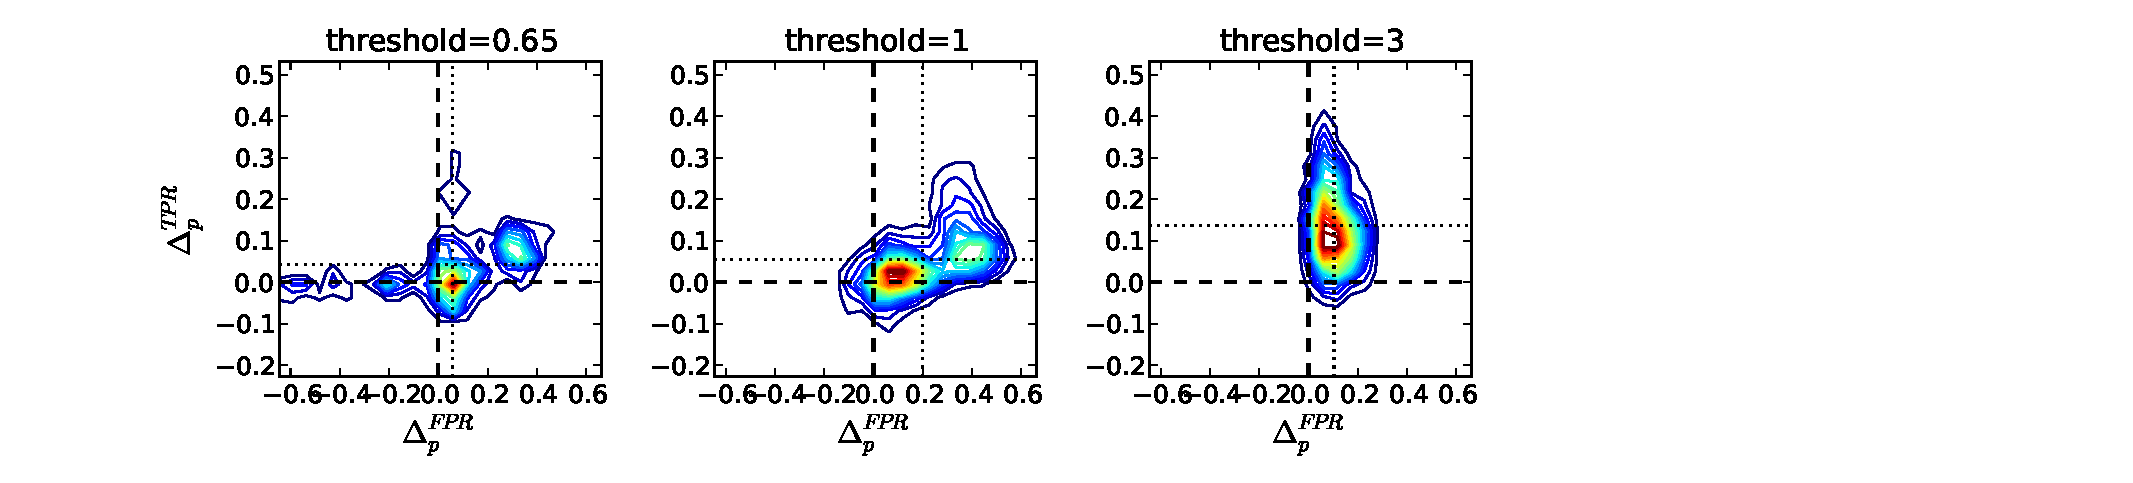
\includegraphics[height=2.5in]{../fig/final/scatter_env/threshold}
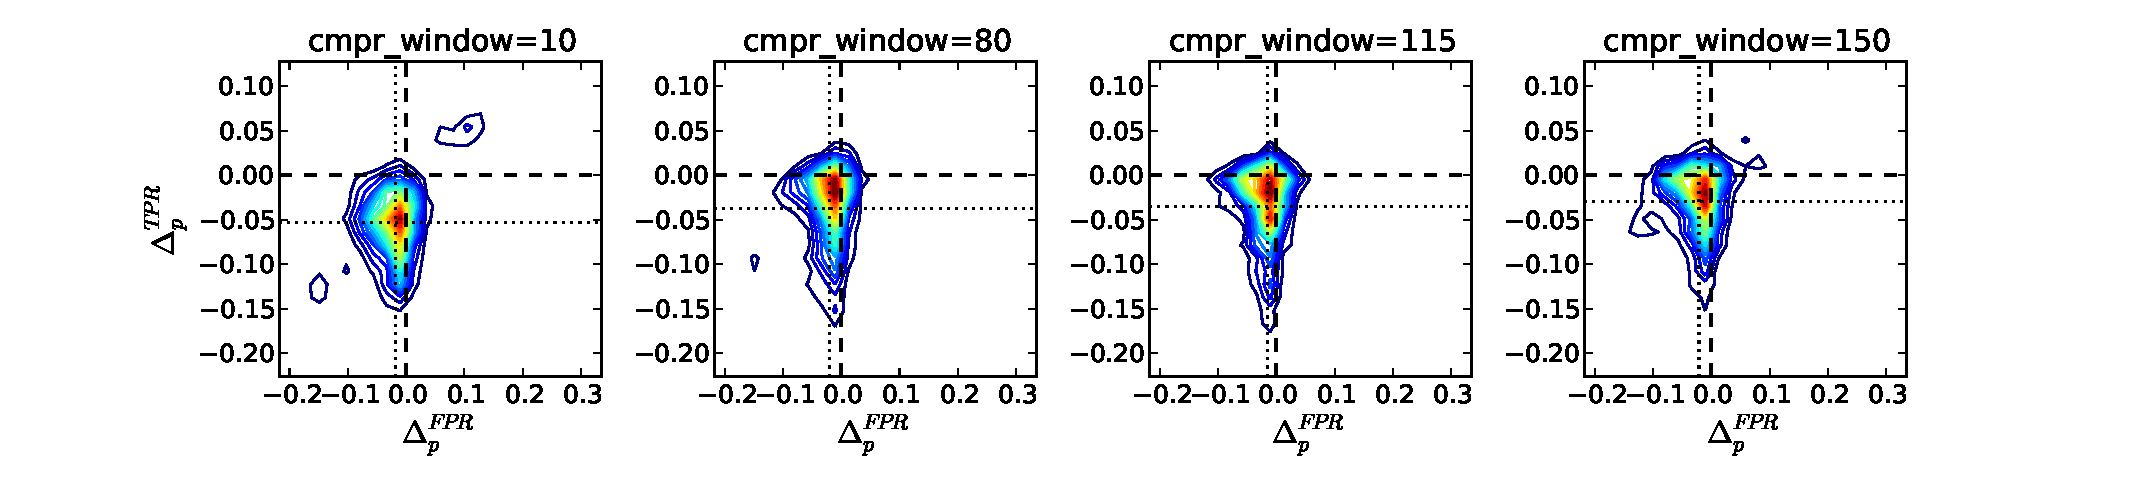
\includegraphics[height=2.5in]{../fig/final/scatter_env/cmpr_window}
\end{center}
\caption{\label{fig:roc_env2}}
\end{figure}

\begin{figure}[!h]
\begin{center}
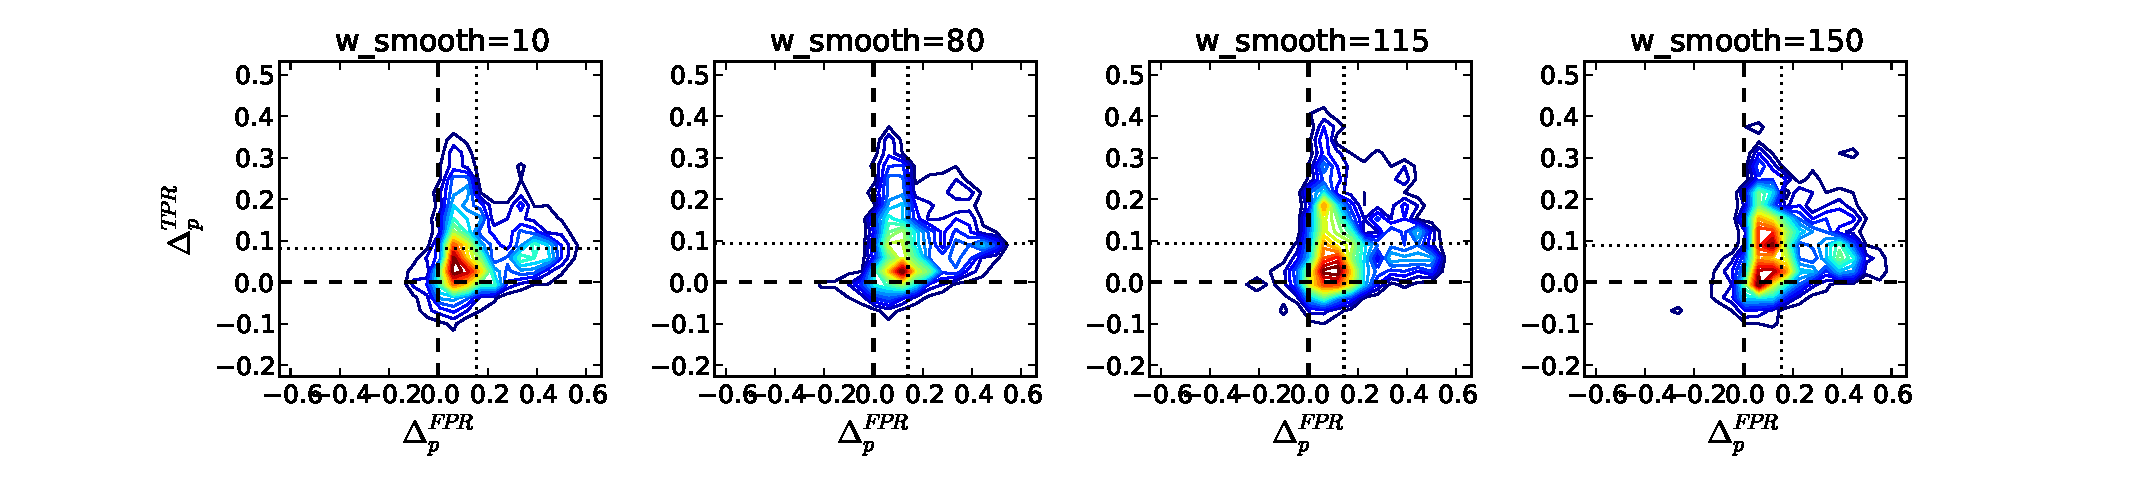
\includegraphics[height=2.5in]{../fig/final/scatter_env/w_smooth}
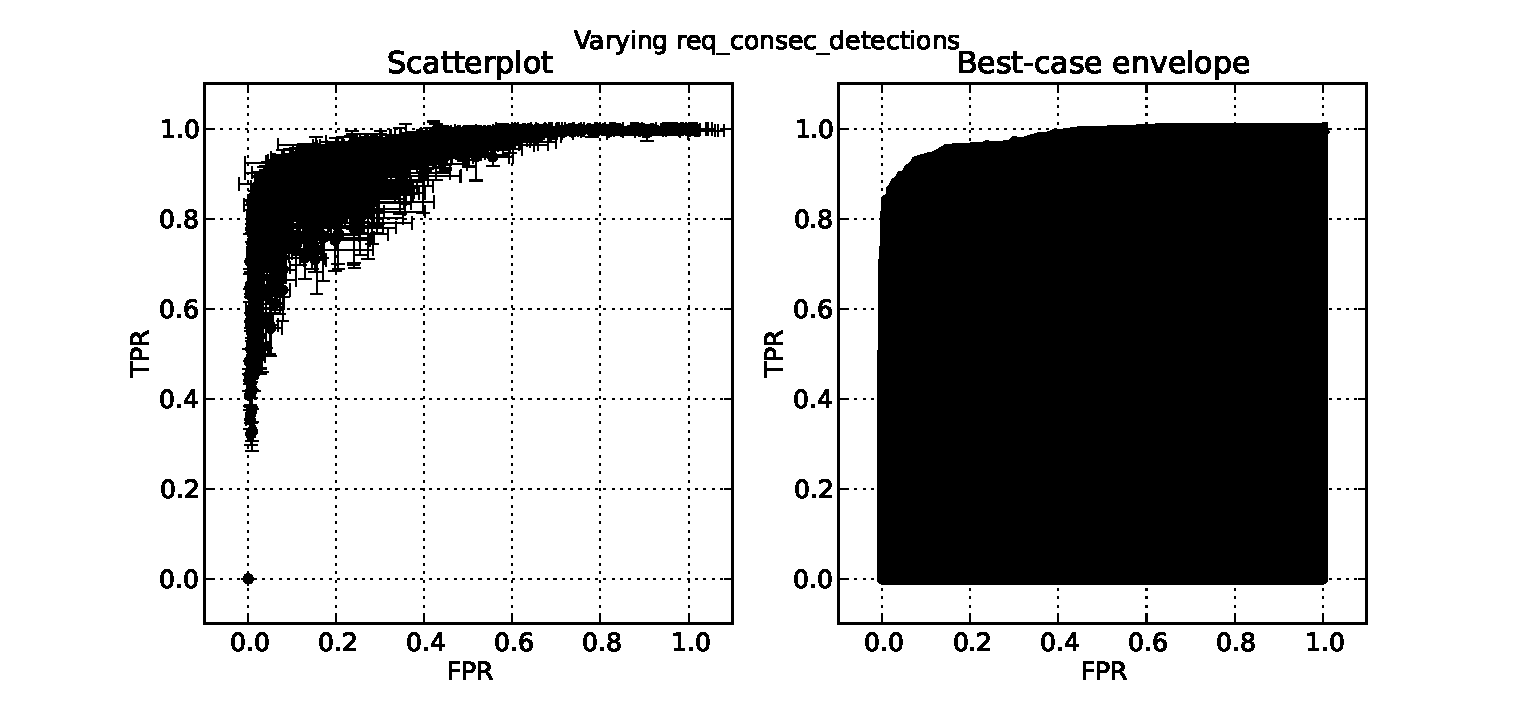
\includegraphics[height=2.5in]{../fig/final/scatter_env/req_consec_detections}
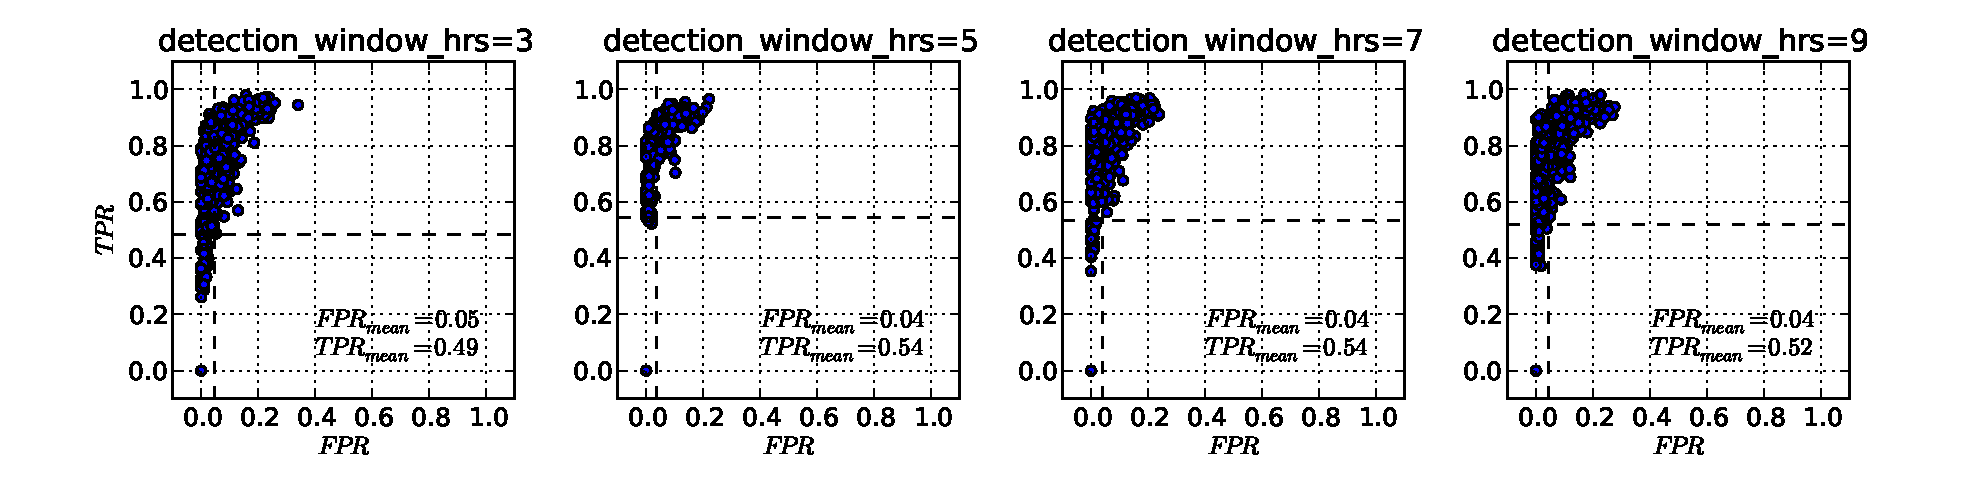
\includegraphics[height=2.5in]{../fig/final/scatter_env/detection_window_hrs}
\end{center}
\caption{\label{fig:roc_env1}}
\end{figure}
\end{comment}

\begin{figure}[!h]
\begin{center}
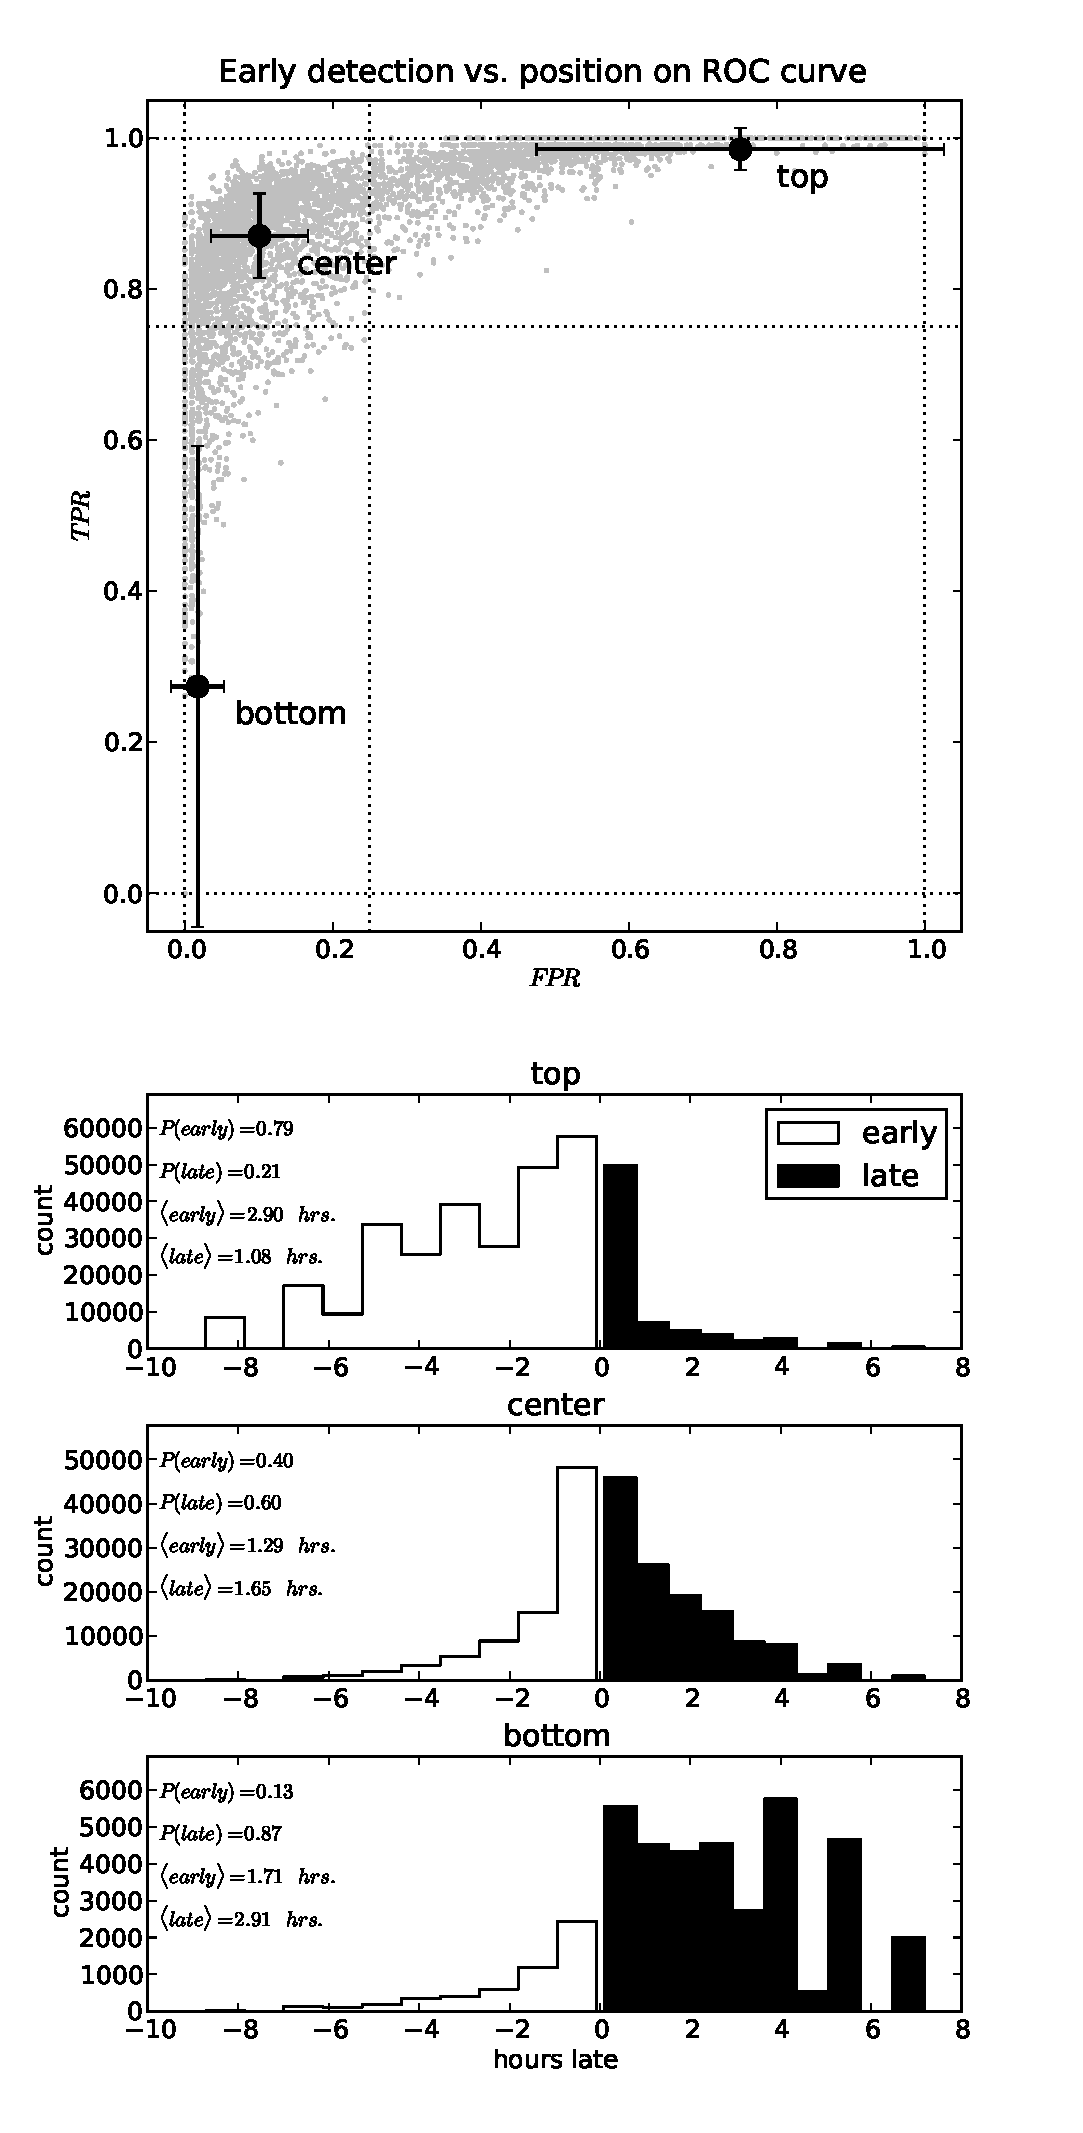
\includegraphics[height=8in]{../fig/final/early_vs_roc}
\end{center}
\caption{\label{fig:early_vs_roc}}
\end{figure}

\clearpage
\section{Examples} %TODO: Call this something better

\begin{figure}[!h]
\begin{center}
\includegraphics[height=2.5in]{../fig/final/detection_examples/danny_welbeck.eps}
\includegraphics[height=2.5in]{../fig/final/detection_examples/barclays.eps}
\end{center}
\caption{\label{fig:examples1} Fast-spreading vs. slow-spreading topics. {\bf
    Top}: English football player Danny Welbeck scores late in the second half
  of the June 15th match between England and Sweden in the Euro 2012, securing a
  3-2 victory for England. The reaction on Twitter is immediate. {\bf Bottom:}
  Ed Miliband, leader of the UK's Labour Party, calls for a criminal
  investigation of Barclays, the global financial services provider, over
  involvement in the Libor fraud scandal. The story stimulates steadily growing
  discussion over the course of the day.}
\end{figure}

\begin{figure}[!h]
\begin{center}
\includegraphics[height=2.5in]{../fig/final/detection_examples/tn/ludacris.eps}
\includegraphics[height=2.5in]{../fig/final/detection_examples/tn/tweetin.eps}
%\includegraphics[height=2.5in]{../fig/final/detection_examples/tn/whooo.eps}
\end{center}
\caption{\label{fig:examples2} Examples of true negatives --- topics that did
  not trend and were not detected as trending. {\bf Top}: Although Ludacris, a
  well-known celebrity, receives constant attention on Twitter, there is no
  anomolous event involving Ludacris that would cause the topic to trend. {\bf
    Bottom}: The word ``tweetin'' is being used as a part of regular speech to
  refer to the act of posting a message on Twitter, and does not constitute a
  trending topic. }
\end{figure}

\begin{figure}[!h]
\begin{center}
\includegraphics[height=2.5in]{../fig/final/detection_examples/fp/dragonfly.eps}
\includegraphics[height=2.5in]{../fig/final/detection_examples/fp/redsn0w.eps}
%\includegraphics[height=2.5in]{../fig/final/detection_examples/tn/whooo.eps}
\end{center}
\caption{\label{fig:examples3} Examples of false positives --- topics that did
  not trend but were detected as trending. {\bf Top}: If the activity of a topic trends
  upward for a sufficiently long time, it may sufficiently resemble the activity
  of topics that trendedand lead to a false detection. {\bf Bottom}: Some false positives
  refer to actual breaking events that happened to not make the Trending Topics
  list on Twitter. The topic ``redsn0w,'' for example, coincides with a new
  release of popular jailbreaking tool for iOS}
\end{figure}

\clearpage
\section{Effect of Parameters}

For each ROC curve, we have a parameter that varies to produce the ROC curve,
which we will call the variable paramter, and a fixed combination of the
remaining paramters, which we will call the constant parameters.

Do we move up or down the curve?

We show how varying a given parameter $p$ trades off $FPR$ for $TPR$ by
computing the discrete derivative of $FPR$ and $TPR$ with respect to $p$. For
each ROC curve, corresponding to the variable parameter $p$ and some fixed
combination of remaining parameters, we compute
\begin{gather}
\Delta_{p,i}^{FPR} = \frac{FPR(p_{i}) - FPR(p_{i-1})}{p_i - p_{i-1}}\\
\Delta_{p,i}^{TPR} = \frac{TPR(p_{i}) - TPR(p_{i-1})}{p_i - p_{i-1}}
\end{gather}
for each ROC curve associated with $p$ and for $i$ ranging from the second to the last value
of $p$ in increasing order. If each point on the ROC curve is produced by
multiple trials, we compute the above for all possible combinations of ROC
curves. Finally, we compute the above across all combinations of fixed
parameters.

The result is a distribution of discrete derivatives of $FPR$ and $TPR$ with
respect to a variable parameter of interest $p$ which highlights the effect of
$p$ on tradeoffs between $FPR$ and $TPR$. We can refer this effect as moving
``up'' the ROC curve, or ``down'' the ROC curve. If most of the mass of
$\Delta_{p}^{FPR}$ and $\Delta_{p}^{TPR}$ is at values greater than 0, then an
increase in $p$ causes a decrease in $FPR$ at the expense of lower $TPR$, moving
down the curve. If, on the other hand, most of the mass is at values less than
zero, an increase in $p$ causes an increase in $TPR$ at the expensive of higher
$FPR$, moving up the curve.

Sometimes, the curve moves neither toward $(0,0)$ (``down the curve'') nor
toward $(1,1)$ (``up the curve'') but toward $(0,1)$ or $(1,0)$. The former
represents an increase in $TPR$ in addition to a decrease in $FPR$ --- a win-win
situation. The latter represents the exact opposite of that --- an increase in
$FPR$ and a decrease in $TPR$.

Note that we did not count $\Delta_p$ for consecutive points at $(0,0)$ or
$(1,1)$ since the $TPR$ and $FPR$ are not free to move any further despite
changes to the variable parameter.

%TODO: Table for deltas. Try showing also deltas for detection time.

%TODO: What parameters contribute to being in the top, bottom. How to show detection time?
\begin{table}
\begin{center}
\begin{tabular}{|l|llllll|}
\hline
& $\langle N_{obs} \rangle$ & $\langle h_{ref} \rangle$ &$\langle \gamma
  \rangle$ & $\langle D_{req} \rangle$ & $\langle \theta \rangle$ & $\langle
  N_{smooth} \rangle$ \\\hline
top & 76.93 & 6.86 & 4.38 & 2.90 & 0.81 & 88.66\\
center & 77.92 & 6.09 & 3.75 & 2.88 & 1.79 & 88.61\\
bottom & 68.76 & 6.83 & 1.81 & 3.70 & 2.69 & 88.10\\
\hline
\end{tabular}
\end{center}
\caption{\label{tbl:roc_pos}}
\end{table}

\section{Recommendations}
